\documentclass[     
	paper=A4,           % Papierformat
	fontsize=12pt,      % Schriftgröße (12pt, 11pt (Standard))
	BCOR=12mm,          % Bindekorrektur, bspw. 1 cm
	DIV=14,             % breiter Satzspiegel
	parskip=half,       % Absatzformatierung s. scrguide 3.1
	headsepline,        % Trennline zum Seitenkopf
	footsepline,       % Trennline zum Seitenfuß
	%normalheadings,    % Überschriften etwas kleiner (smallheadings)
	listof=totoc,       % Tabellen & Abbildungsverzeichnis ins Inhaltsverzeichnis
	%bibtotoc,          % Literaturverzeichnis im Inhalt
	%draft              % Überlangen Zeilen in Ausgabe gekennzeichnet
	footinclude=false,  % Fußzeile in die Satzspiegelberechnung einbeziehen
	headinclude=true,   % Kopfzeile in die Satzspiegelberechnung einbeziehen
	final,              % draft beschleunigt die Kompilierung
	ngerman
]{scrartcl}

%---------------FRONT PAGE CONFIG----------------%
\newcommand{\documentType}{TYPE}
\newcommand{\submissionDate}{dd.mm.yyyy}
\newcommand{\documentTitle}{TITLE}
\newcommand{\documentSubTitle}{-}
\newcommand{\documentAuthor}{NAME}
\newcommand{\documentAuthorAdress}{ADRESS}
\newcommand{\documentExaminer}{EXAMINER}
\newcommand{\assosiatedCompany}{COMPANY}
\newcommand{\matriculationNumber}{matrknumber}
\newcommand{\studygroup}{group}

%Pdf
\pdfinfo{ /ModDate ()  /CreationDate () }
\pdftrailerid{}


%-----------BASIC IMPORTS----------------%
\usepackage[utf8]{inputenc}
\usepackage{graphicx}
\usepackage{pdfpages}
\usepackage{mathptmx}
\usepackage{amsmath}
\usepackage[]{xcolor}
\usepackage{tabularx} % tables
\usepackage{fixfoot}
\usepackage{rotating}
\usepackage{float}
\usepackage{ltablex}
\usepackage{tikz}
\usepackage{color, colortbl} 
\usepackage{url} %url handling (\url{https://...})
\usepackage{paralist} % lists without spacing
\usepackage[activate={true,nocompatibility},final,tracking=true,kerning=true,spacing=true,factor=1100,stretch=10,shrink=10]{microtype} %enhances readablity
\usepackage{listings}
\usepackage[printonlyused]{acronym}

%-----------Formalia---------------------%
\usepackage[a4paper, left=4cm, right=2cm, top=2.5cm, bottom=2.5cm]{geometry}
\usepackage[T1]{fontenc}
\usepackage[utf8]{inputenc}
\usepackage[ngerman]{babel}
\usepackage{lmodern} %Latin modern font
\usepackage[onehalfspacing]{setspace} % Line spacing
\usepackage[babel,german=quotes]{csquotes} %german quotes ("")
\usepackage[stable, multiple]{footmisc}
\usepackage[format=hang, font={footnotesize, sf}, labelfont=bf, justification=raggedright,singlelinecheck=false]{caption} %captions in tables and images


%SETTINGS FOR FOMALIA
\addtokomafont{disposition}{\rmfamily}
%\captionsetup[table]{name={\rmfamily Tabelle}}
%\captionsetup[listing]{name={\rmfamily Listing}}
%\captionsetup[figure]{name={\rmfamily Abbildung}}
\DeclareCaptionFont{quack}{\rmfamily}
\parindent 0pt
\setcounter{secnumdepth}{4}
\setcounter{tocdepth}{3}
\lstset{
	breaklines=true,
	postbreak=\raisebox{0ex}[0ex][0ex]{\ensuremath{\color{red}\hookrightarrow\space}},
	numbers=left,
	inputencoding=utf8,
	emptylines=1,
	showlines=true
}

%LIstings
\definecolor{groovyblue}{HTML}{0000A0}
\definecolor{groovygreen}{HTML}{008000}
\definecolor{darkgray}{rgb}{.4,.4,.4}

%\lstdefinelanguage{base}[]{SQL}{
%	keywordstyle=\color{groovyblue}\bfseries,
%	stringstyle=\color{groovygreen}\ttfamily
%}

%-----------Fancy Header----------------%
%\usepackage{fancyhdr}
\usepackage{scrlayer-scrpage}
\clearpairofpagestyles 
\KOMAoptions{
   headsepline = true,
   footsepline = false,
   plainfootsepline = true,
}
\ohead{\headmark}
\ofoot*{\pagemark}


%-----------BibTex----------------%
\usepackage{etoolbox} %is required
\usepackage[
    style=authoryear,
    %citestyle=authoryear-fhdw,
    giveninits=false, %complete first names
    natbib=true,
    urldate=long,
    seconds=true,
    dashed=false,
    maxcitenames=3,
    maxbibnames=99,
    backend=biber
]{biblatex}
\addbibresource{Directories/Library.bib}

%Graphics
\graphicspath{{Assets/Images/}}
\usetikzlibrary{arrows,positioning,calc,intersections,decorations.markings,fit,chains}
\tikzset{
	base/.style={
			draw,
			rectangle,
			align=center
		}
}
\microtypecontext{spacing=nonfrench}

\usepackage{hyperref}
\hypersetup{pdfinfo={ Creator={}, Producer={} }}
\usepackage[ngerman,capitalise]{cleveref} % better referencing (has to be imported after hyperref)


%Commands
\newcommand{\todo}[1]{\textbf{\textsc{\textcolor{red}{(TODO: #1)}}}}
\newcommand{\new}[1]{\textbf{\textsc{\textcolor{green}{(Marker: #1)}}}}

\newcommand{\imgwidth}{\linewidth-2\fboxsep-2\fboxrule}

\newcommand{\sees}[2][sec]{\hyperref[#1:#2]{ \autoref*{#1:#2}}}
\newcommand{\seesf}[1]{\see[fig]{#1}}
\newcommand{\seesl}[1]{\see[lst]{#1}}
\newcommand{\seesi}[1]{\see[itm]{#1}}

\newcommand{\see}[2][sec]{\hyperref[#1:#2]{siehe \autoref*{#1:#2}}}
\newcommand{\seef}[1]{\see[fig]{#1}}
\newcommand{\seel}[1]{\see[lst]{#1}}
\newcommand{\seei}[1]{\see[itm]{#1}}

\newcommand{\seeb}[2][sec]{\hyperref[#1:#2]{(siehe \autoref*{#1:#2})}}
\newcommand{\seelb}[1]{\seeb[lst]{#1}}
\newcommand{\seefb}[1]{\seeb[fig]{#1}}
\newcommand{\seeib}[1]{\seeb[itm]{#1}}

\newcommand{\seep}[3][sec]{\hyperref[#1:#2]{siehe #3 in \autoref*{#1:#2}}}
\newcommand{\seepf}[2]{\seep[fig]{#1}{#2}}
\newcommand{\seepl}[2]{\seep[lst]{#1}{#2}}
\newcommand{\seepi}[2]{\seep[itm]{#1}{#2}}

\newcommand{\seepb}[3][sec]{\hyperref[#1:#2]{(siehe #3 in \autoref*{#1:#2})}}
\newcommand{\seepbf}[2]{\seepb[fig]{#1}{#2}}
\newcommand{\seepbl}[2]{\seepb[lst]{#1}{#2}}
\newcommand{\seepbi}[2]{\seepb[itm]{#1}{#2}}

\newcommand{\seea}[1]{\hyperref[app:#1]{siehe Anhang~\ref*{app:#1}}}
\newcommand{\seeab}[1]{\hyperref[app:#1]{(siehe Anhang~\ref*{app:#1})}}
\newcommand{\seeabd}[1]{\hyperref[app:#1]{(Details siehe Anhang~\ref*{app:#1})}}
\newcommand{\seepa}[2]{\hyperref[app:#1]{siehe #2 in Anhang~\ref*{app:#1}}}
\newcommand{\seepba}[2]{\hyperref[app:#1]{(siehe #2 in Anhang~\ref*{app:#1})}}

\newcommand{\seelz}[2]{\hyperref[lst:#1]{siehe \autoref*{lst:#1}, Zeile #2}}
\newcommand{\seelbz}[2]{\hyperref[lst:#1]{(siehe \autoref*{lst:#1}, Zeile #2)}}

\newcommand{\seeplz}[3]{\hyperref[lst:#1]{siehe #3 in \autoref*{lst:#1}, Zeile #2}}
\newcommand{\seeplbz}[3]{\hyperref[lst:#1]{(siehe #3 in \autoref*{lst:#1}, Zeile #2)}}


\newcommand{\ar}[2][sec]{\autoref{#1:#2}}
\newcommand{\arl}[1]{\ar[lst]{#1}}
\newcommand{\arf}[1]{\ar[fig]{#1}}
\newcommand{\ari}[1]{\ar[itm]{#1}}

\newcommand{\arb}[2][sec]{(\autoref{#1:#2})}
\newcommand{\arfb}[1]{\arb[fig]{#1}}
\newcommand{\arlb}[1]{\arb[lst]{#1}}
\newcommand{\arib}[1]{\arb[itm]{#1}}

\newcommand{\arlz}[2]{\hyperref[lst:#1]{\autoref*{lst:#1}, Zeile #2}}
\newcommand{\arlbz}[2]{\hyperref[lst:#1]{(\autoref*{lst:#1}, Zeile #2)}}


\newcommand{\ctapp}[2]{\footnote{\hyperref[app:#1]{#2}}}

\newcommand{\cit}[3]{\footcite[#2][#3]{#1}}
\newcommand{\ct}[2][]{\cit{#2}{#1}{}}
\newcommand{\vg}[1]{\ct[vgl.]{#1}}

\newcommand{\ctsep}{\textsuperscript{,}}
\newcommand*{\authormark}{}
\newcommand*{\markauthor}[1]{%
   \renewcommand{\authormark}{#1}%
   \ignorespaces
}

%Sources, Images and Tables
\newcommand{\source}[1]{{\vspace{-1mm}\\\footnotesize\textsf{\rmfamily\textbf{Quelle:}} \textsf{\rmfamily#1}\par}}
\newcommand{\sourcelst}[1]{{\vspace{-6mm}\\\footnotesize\textsf{\rmfamily\textbf{Quelle:}} \textsf{\rmfamily#1}\par}}


%BEGIN OF DOCUMENT%

\begin{document}

%---------------Frontpage---------------%
\begin{titlepage}
    \begin{center}
        %University-Logo (Assets/Images/)
        
\includegraphics[scale=1.20]{FHDW.jpg}\\\vspace{0.7cm}

        %Document type
        \Huge{\bfseries\documentType}\\
        ~\vspace{.3cm}

        %Title of the document
        \LARGE{\documentTitle}\\
        ~\vspace{1.3cm}

        \large{
            %Document author
            Erstellt von:\\
            \vspace{1.5mm}
            \documentAuthor \\

            %adress of the author            
            \documentAuthorAdress \\
            \vspace{.5cm}

            %Uni-specific values
            Matrikelnummern: \matriculationNumber\\
            Studiengruppe: \studygroup \\

            \vspace{1cm}

            %Examiner of the document
            Gutachter: \\
            \vspace{1.5mm}
            \documentExaminer \\

            \vspace{.5cm}

            %Date of submission
            Abgabetermin: \\
            \vspace{1.5mm}
            \submissionDate
        }
    \end{center}
\end{titlepage}
\pagenumbering{Roman}

%-------------Sperrvermerk--------------%
\section*{Sperrvermerk}
\addcontentsline{toc}{section}{Sperrvermerk}
\ohead*{Sperrvermerk}

Diese \documentType{} enthält vertrauliche Informationen über die Firma \assosiatedCompany. 
Die Weitergabe des Inhalts dieser Arbeit (auch in Auszügen) ist untersagt. 
Es dürfen keinerlei Kopien oder Abschriften - auch nicht in digitaler Form - angefertigt werden. 
Auch darf diese Arbeit nicht veröffentlicht werden und ist 
ausschließlich dem Prüfer, Mitarbeitern der Verwaltung und Mitgliedern des Prüfungsausschusses sowie auf Nachfrage einer Evaluierungskommission zugänglich zu machen. 
Personen, die Einsicht in diese Arbeit erhalten, verpflichten sich, über die Inhalte dieser Praxisarbeit und all ihren Anhängen keine Informationen, 
die die \assosiatedCompany{} betreffen, gegenüber Dritten preiszugeben. Ausnahmen bedürfen der schriftlichen Genehmigung der \assosiatedCompany.
\newpage


%----------Executive Summary------------%
\section*{Executive Summary}
\addcontentsline{toc}{section}{Executive Summary}
\ohead*{Executive Summary}

Executive Summary text.

\newpage

%--------------Directories--------------%
\ohead*{Inhaltsverzeichnis}
\tableofcontents
\newpage % Table of contents
\section*{Abkürzungsverzeichnis}
\ohead*{Abkürzungsverzeichnis}
\addcontentsline{toc}{section}{Abkürzungsverzeichnis}

\begin{acronym}
    
\end{acronym}
\newpage %Abkürzungsverzeichnis
\ohead*{Tabellenverzeichnis}
\listoftables
\newpage % Table of tables !?
%\ohead*{Quelltextverzeichnis}
\lstlistoflistings
\newpage %Quelltextverzeichnis

\ohead*{\leftmark}
\pagenumbering{arabic}

%%%%%%%%%%%%%%%%%%%%%%%%%%%%%%%%%%%%%%%%
%%%%%            Content         %%%%%%%
%%%%%%%%%%%%%%%%%%%%%%%%%%%%%%%%%%%%%%%%



%%%%%%%%%%%%%%%%%%%%%%%%%%%%%%%%%%%%%%%%
%%%%%       End of Content       %%%%%%%
%%%%%%%%%%%%%%%%%%%%%%%%%%%%%%%%%%%%%%%%

%-----------Source Directory------------%
\section*{Quellenverzeichnis}
\addcontentsline{toc}{section}{Quellenverzeichnis}
\ohead*{Quellenverzeichnis}

\newpage

%--------Ehrenwörtliche Erklärung-------%
\section*{Ehrenwörtliche Erklärung}
\addcontentsline{toc}{section}{Ehrenwörtliche Erklärung}
\ohead*{Ehrenwörtliche Erklärung}

Hiermit erkläre ich, Fabian Tilmans, dass ich die vorliegende \documentType{} selbständig angefertigt habe. 
Es wurden nur die in der Arbeit ausdrücklich benannten Quellen und Hilfsmittel benutzt. 
Wörtlich oder sinngemäß übernommenes Gedankengut habe ich als solches kenntlich gemacht. 
Diese Arbeit hat in gleicher oder ähnlicher Form noch keiner Prüfungsbehörde vorgelegen.
\vspace{20mm}

Burscheid, den 01.05.2022
\vspace{10mm}

\hspace*{-0.5cm}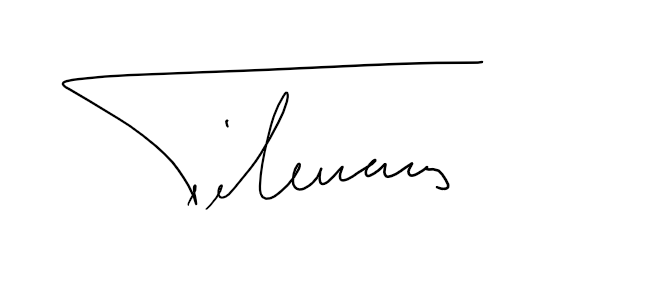
\includegraphics[width=0.3\textwidth]{Unterschrift.png}
\hspace{8cm}\\\documentAuthor{}

\end{document}